\chapter{Extended Neyman Pearson Test}
This chapter will start by introducing the Extended Neyman Pearson Framework. A few properties concerning ENP test will be shown. The limitation of ENP framework will come after that. Following that is a section which detailedly present Modified Extended Neyman Pearson (MENP) Framework. The new scheme aims to achieve the largest probability of detection under any possible probability of false alarm constraints. Then an algorithm which aims at achieving the MENP parameters will be reviewed. Computer simulation results, which illustrate the performance of the algorithm, will be presented. 

\section{Extended Neyman Pearson Hypotheses Testing}
The theories of hypotheses testing have been a subject of continuous studies, and have found applications in various fields such as radar systems, spectrum sensing for cognitive communication systems, and in  medical science \cite{srinivasan1986distributed,  ma2008soft, spielman1973refutation}. One type of hypotheses testing problem can be abstracted as  follows: assume $M+1$  hypotheses $H_0$, $H_1$, ..., $H_{M}$, inducing $M+1$  Probability Density Functions (PDFs) on the observable $Y$,
\begin{equation}
\label{equ:hypothesis}
\begin{split}
H_0:\;\;\;\;\;\;\;\;\;&Y \sim f_0(y) \\
H_1:\;\;\;\;\;\;\;\;\;&Y \sim f_1(y)\\
&......\\
H_M:\;\;\;\;\;\;\;\;\;&Y \sim f_M(y)\\
\end{split}
\end{equation}

Based on $y$, a realization of $Y$, the detector needs to decide whether or not it comes from $f_0(y)$. A framework for solving this problem for $M=1$ was introduced in \cite{neyman1933problem} and it is commonly known as Neyman Pearson (NP) testing. The theory of NP testing was further developed for $M \geq 2$ in \cite{wald1939contributions} and \cite{dantzig1951fundamental}.  A comprehensive exposition of such generalized NP testing can be found in \cite{LehmannTest}.

\noindent  \textbf{The Extended Neyman Pearson (ENP) Lemma:}

\textit{
Let $f_0(x), f_1(x), ..., f_{m}(x)$ be real Borel measurable functions  defined on finite dimensional  Euclidean space $\mathcal{R}$ such that $\int \limits_R | f_i(x)|\mathrm{d}x < \infty (i=0, 1,...,M)$.  Suppose that for given constants $c_1,...,c_M$ there exists a class of subsets $\mathcal{S}$, denoted $\mathcal{C}_\mathcal{S}$, such that for every $\mathcal{S} \in \mathcal{C}_\mathcal{S}$ we have
\begin{equation}
\label{one}
\int\limits_\mathcal{S} f_i(x)\mathrm{d}x = c_i, \;\;\;\;\;\;i=1,...,M
\end{equation}
Then:
%No. 1
\\\textnormal{(\rmnum{1})} Among all members of $\mathcal{C}_\mathcal{S}$ there exists one that maximizes
\[
\int \limits_\mathcal{S} f_{0}(x)\mathrm{d}x.
\]
%No.2
\\\textnormal{(\rmnum{2})} A sufficient condition for a member of $\mathcal{C}_\mathcal{S}$ to maximize
\[
\int \limits_\mathcal{S} f_{0}(x)\mathrm{d}x.
\]
is the existence of constants $k_1,...,k_M$ such that
\begin{equation}
\label{2}
f_{0}(x)>\sum\limits_{j=1}^M k_j f_j(x)\;\;\;\;\text{when $x \in \mathcal{S}$}
\end{equation}
\begin{equation}
\label{3}
f_{0}(x)<\sum\limits_{j=1}^M k_j f_j(x)\;\;\;\;\text{when $x \notin \mathcal{S}$}
\end{equation}
%No. 3
\\\textnormal{(\rmnum{3})} If a member of $\mathcal{C}_\mathcal{S}$ satisfies  \textnormal{(\ref{2})} and \textnormal{(\ref{3})} with $k_1,...,k_M\geq0$, then it maximizes
\begin{equation}
\label{4}
\int \limits_\mathcal{S} f_{0}(x)\mathrm{d}x
\end{equation}
among all $\mathcal{S} \in \mathcal{C}_{\mathcal{S}}$ satisfying
\begin{equation}
\label{5}
\int \limits_\mathcal{S} f_i(x)\mathrm{d}x\leq c_i,\;\;\;\;i=1,...,M.
\end{equation}
%no. 4
\\\textnormal{(\rmnum{4})} The set $M$ of points in $M$-dimensional space whose coordinates are 
\begin{equation}
(\int_{\mathcal{S}}f_1(x)\mathrm{d}x, ..., \int_{\mathcal{S}}f_M(x)\mathrm{d}x)
\end{equation}
for any $\mathcal{S}$ is convex and closed. If $(c_1, ..., c_M)$ is an inner point of $M$, then a  necessary condition for a member of $\mathcal{C}_\mathcal{S}$ to maximize 
\[
\int \limits_\mathcal{S} f_{0}(x)\mathrm{d}x.
\]
is that there exist $M$ constants $k_1, ..., k_M$ such that \eqref{2} \eqref{3} holds a.e..
}

The associated probability of detection, $P_d$ and false alarms $P_{f_i}$ for a certain subset $\mathcal{S}$ are defined as
\cite{neyman1933problem}, 
\begin{equation}
\begin{split}
P_d &= P(H_0 | H_0) = \int_{\mathcal{S}}f_0(x)\mathrm{d}x\\
P_{f_1} &= P(H_0 | H_1) = \int_{\mathcal{S}}f_1(x)\mathrm{d}x\\
&......\\
P_{f_M} &= P(H_0 | H_M) = \int_{\mathcal{S}}f_M(x)\mathrm{d}x
\end{split}
\end{equation}

 Define the step function
\begin{equation}
   \label{equ: step function}
   u(x) = \begin{cases}
     0\;\;\;\;\;\;&x < 0\\
     0.5\;\;\;\;\;\;&x=0\\
     1\;\;\;\;\;\;&x>0\,,
   \end{cases}
\end{equation}
then for a subset $\mathcal{S}$ satisfying \eqref{2} and \eqref{3} we have:
\begin{equation}
\label{equ: pf and pd}
\begin{split}
&P_d = \int_{-\infty}^{\infty} u(f_0(x) - \sum_{j=1}^{M}k_jf_j(x)) f_0(x)\mathrm{d}x	\,, \\
&P_{f_i} = \int_{-\infty}^{\infty} u(f_0(x) - \sum_{j=1}^{M}k_jf_j(x)) f_i(x) \mathrm{d}x\;\;	 i=1, 2, ..., M\,.
\end{split}
\end{equation}
The relationship between $P_d$ and $P_{f_i}$ can be represented by Receiver Operating Characteristic (ROC) surface \cite{LehmannTest}.

From to \eqref{2} \eqref{3}, the ENP Decision rule $\delta$ is

\begin{equation}
\label{equ: decision rule}
\delta: f_0(x) \substack{H_0 \\ \geq \\ < \\ \bar{H}_0}  \sum_{j=1}^{M} k_jf_j(x)
\end{equation}

From the  \textbf{ENP Lemma}, $\delta$  achieves the largest $P_d$ under the constraints $P_{f_i} = c_i (i = 1, 2, ..., M)$.
When $M=1$, it achieves the largest $P_d$ under the constraint $P_f \leq c$ \cite{LehmannTest}, which is the well known and commonly used form.

% notes from Prof. Leib.
For applications in spectrum sensing, $H_0$ denotes the hypothesis that the channel is free and $H_m \;(m=1, ..., M)$ corresponds to the hypothesis that the channel is occupied by the $m$-th primary signal. Although we have $M$ hypotheses, we intend to determine if the channel is free or not. Hence the problem is to find a binary test of deciding $H_0$ versus $\bar{H}_0$ such that $P_d$ is maximized under the constraints $P_{f_m} \leq c_m$ $m = 1, ..., M$. In context of spectrum sensing, $1-P_{f_m}$ can be interpreted as the protection level of the $m-$th primary signal. The larger is this protection level, the smaller is the probability that when the $m-$th signal is active, the test will not detect it and will declare the channel free. In context of spectrum sensing the solution of the ENP problem maximizes the probability of detecting a free channel under a constraint on the protection level for each primary signal. The protection levels of primary signals can be different and they are guaranteed.

\section{Properties of ENP Testing}
In this section, we will provide an example and three lemmas to present the properties of ENP test. 

\subsection{An Example of ENP Test}
Assume three hypotheses given as:
\begin{equation}
\begin{split}
H_0:\;\;\;\;&Y \sim \mathcal{N}(0, 5)\\
H_1:\;\;\;\;&Y \sim \mathcal{N}(0, 3)\\
H_2:\;\;\;\;&Y \sim \mathcal{N}(1, 5)
\end{split}
\end{equation}
where $\mathcal{N}(\mu, \epsilon^2)$ denotes a Gaussian PDF with mean $\mu$ and variance $\epsilon^2$. By conducting an exhaust search on the grid of $k_1, k_2$ (range from $-30$ to $30$ with step $0.1$), an ROC surface is achieved  and presented in Fig. \ref{fig: 2.1}. 

\begin{figure}[!t]
\centering
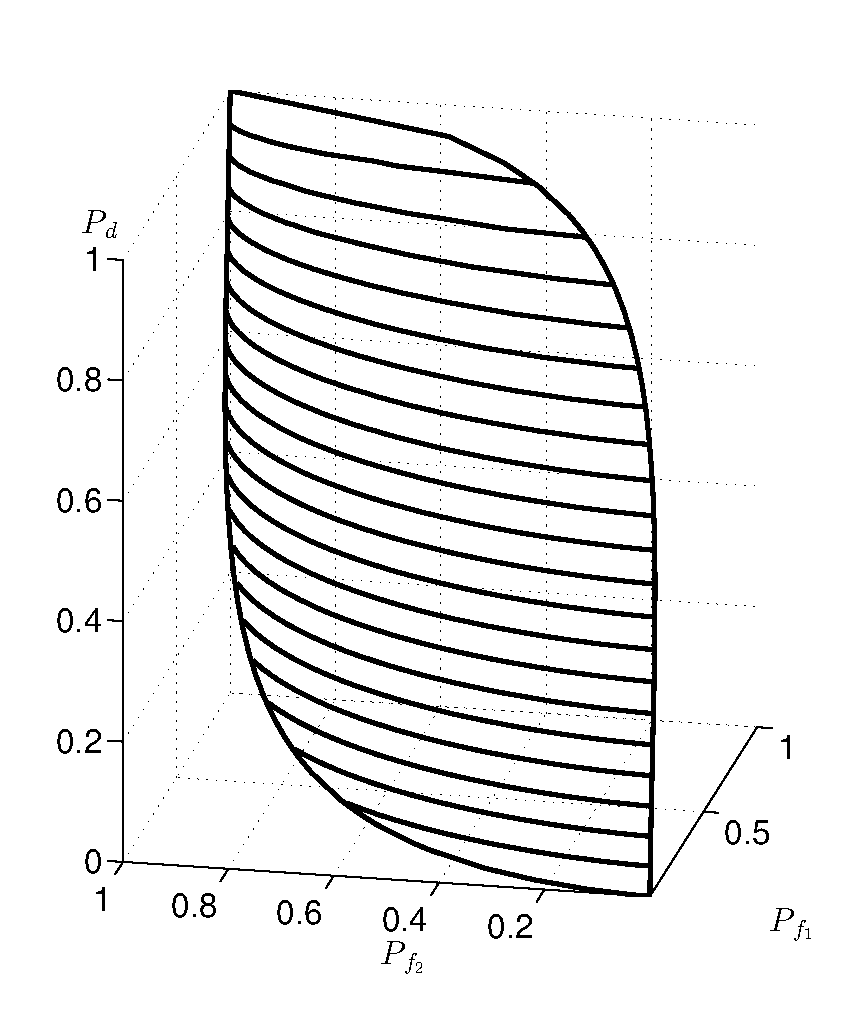
\includegraphics[width = 12cm]{c21.eps}
\caption{The ROC surface for $k_1$, $k_2$ range from $-30$ to $30$ with step $0.1$}
\label{fig: 2.1}
\end{figure}

It is interesting to observe that under the framework of ENP test, for a given $(P_{f_1}, P_{f_2})$, $P_d$ does not always exit. Recall in the case of binary hypotheses testing (Traditional Neyman Pearson Test), for any given $P_f$, there is a corresponding $P_d$. 

Now let us consider points $A$ and $B$ on the ROC surface, which are marked with $\blacksquare$ and $\diamondsuit$, respectively.  The coordinate of point $A$ is $(P_{f_1}, P_{f_2}, P_d) = (0.0841, 0.1761, 0.2868)$; and the coordinate of point $B$ is  $(P_{f_1}, P_{f_2}, P_d) = (0.0807, 0.0570, 0.3344)$. We can see even through $P_{f_1}$ and $P_{f_2}$ of point $A$ is larger than that of point $B$, the probability of detection of point $A$ is  smaller than that of point $B$.  
Unlike NP test, where $P_d$ is always non-decrease when $P_f$ increases, in the case of multiple hypotheses testing (Extended Neyman Pearson Test), $P_d$ is not always an non-decreasing function of  $P_{f_i}$ ($i=1, ..., M$).

Finally we consider in $P_{f_1} = 0.7291$ and $P_{f_2} = 0.9454$, the corresponding point on ROC surface is denoted by point $C$ with mark $\ast$. By using Matlab, we can get the value of  $P_d$ is $0.3819$. 

Finally we consider point $C$ on the ROC surface, which is marked by $\ast$. The coordinate of point $C$ is $(P_{f_1}, P_{f_2}, P_d) = (0.7291, 0.9454, 0.3819)$. We can observe, in this case the value of $P_d$ is smaller than the value of $P_{f_1}$ and $P_{f_2}$, i.e. under the framework of ENP Test, $P_d \geq P_{f_i}$  ($i = 1, ..., M$) does not always hold (Qian Zhang arrives at the same conclusion in  \cite{zhang1999design, zhang2000efficient}). 

\subsection{Three Lemmas concerning ENP Test}


We consider now several properties for the ENP test, embodied by three lemmas with proof placed in the appendix A, B and C.

\noindent \textbf{Condition 1}
\textit{
\noindent Let $f_i(x) \;\;i=0, 1, ..., M$ be the PDF induced by hypothesis $H_i$, and define $g(x) = f_0(x) - \sum_{j=1}^{M} k_jf_j(x)$ where $k_i$  ($i = 1, 2, ..., M$) are real numbers. Let $\mathcal{D} \in \mathbb{R}$ be an open set such that $\int_{\bar{\mathcal{D}}}f_i(x)=0\;\;i = 1, 2, ..., M$. Furthermore,  if $x_0$ is a solution  for $g(x) = 0 \;\;(x \in \mathcal{D})$, there exists an integer $n$ such that  the $n$ order derivative of $g(x_0)$ is not equal to zero $(g^{(n)}(x_0) \neq 0)$.
}

\noindent \textbf{Lemma 1}
\textit{
\noindent Under}
\textbf{Condition 1}
\textit{, let $\mathbf{P}$ be a point with coordinate $(P_d, P_{f_1}, ..., P_{f_M})$ on the ROC surface of the EPN test. If there exists a tangent hyperplane at $\mathbf{P}$, then its normal is parallel to the vector $\mathbf{n} = (-1, k_1, ..., k_M)$, where $k_i$ are the parameters of the ENP test achieving $\mathbf{P}$.
}

\noindent \textbf{Lemma 2}
\textit{
\noindent
Under}
\textbf{Condition 1}
\textit{, let $\mathbf{P}$ be a point on the ROC surface, $\frac{\partial P_d}{\partial P_{f_i}} \bigg|_P = k_i$, where $k_i$ are the parameters of ENP test achieving $\mathbf{P}$.
}

\noindent \textbf{Lemma 3}
\noindent \textit{
    Let $f_0$, $f_1$, ..., $f_M$ be PDFs defined on set $\mathcal{D}$ and $f_i(x) \neq 0$ holds a.e. $\mathcal{D}$ ($i=0, 1,..., M$). Suppose that for given constants $c_1, ..., c_M \in (0, 1]$ there exists a class of decision rules $\delta$, denote $\mathcal{C}_\delta$, such that for every $\delta \in \mathcal{C}_\delta$, we have $P_{f_i} \leq c_i$.  Then:
%No. 1
%\\\textnormal{(\rmnum{1})} Among all members of $\mathcal{C}_\mathcal{S}$ there exists one that maximizes $P_d$.
%No.2
\\ If  $\delta^{\ast}$ is a member of $\mathcal{C}_\delta$ that maximum $P_d$, then there exists non-negative constants $k_1, ..., k_M$ such that 
\[
x \in H_0 \;\;\;\;\textit{when}\;\;\;\;f_0(x) > \sum_{i=1}^{M}k_if_i(x)
\]
\[
x \notin H_0 \;\;\;\;\textit{when}\;\;\;\;f_0(x) < \sum_{i=1}^{M}k_if_i(x)
\]
}

\section{Modified Extended Neyman Pearson Testing}
%define \JUDGEMENT
\def \JUDGEMENT{u(f_0(x) - \sum_{j=1}^{M}k_j f_j(x))}
Before we proceed, we will define some notations for presentation.
Define $\mathbf{c}^T = [c_1, c_2, ..., c_M]$, $\mathbf{a}^T=[a_1, a_2, ..., a_M]$, $\mathbf{k}^T = [k_1, k_2, ..., k_M]$ and  $\mathbf{P}_f^T = [P_{f_1}, P_{f_2}, ..., P_{f_M}]$. Let
$F(\mathbf{a})$ denote the largest $P_d$ under the constraints $P_{f_i} = a_i\;\;i = 1, ..., M$.
$G(\mathbf{c})$ denote the largest $P_d$ under the constraints $P_{f_i} \leq c_i\;\;i = 1, ..., M$.
Also define the set $\mathcal{A}_\mathbf{c} = \{
  \mathbf{P}_f | 0 \leq P_{f_i} \leq c_i
  \;\;i=1, 2, ..., M\}\,.
$ and set $\alpha^+ \triangleq \{\mathbf{P}_f | P_{f_i} = \int_{-\infty}^{\infty} \JUDGEMENT f_i(x) \mathrm{d}x, \text{where\;\;} k_i \geq 0 \;\;i=1, ..., M\}$.
Let $\mathbf{A}$ and $\mathbf{B}$ denote two vectors. 
By $\mathbf{A} \leq \mathbf{B}$, $\mathbf{A} = \mathbf{B}$ and  $\mathbf{A} \geq \mathbf{B}$ we mean that every element of $\mathbf{A}$ is no larger than, equal to and no smaller than its corresponding element of $\mathbf{B}$, respectively. 

In practice (e.g. spectrum sensing in CR communication system), the following problem needs to be solved,

      \begin{equation}
      \label{equ: problemstate}
      \begin{split}
      \max\;\;\;\;\;\;&P_d\\
      \text{s.t.}\;\;\;\;\;\;&\mathbf{P}_f \leq \mathbf{c}
      \end{split}
      \end{equation}

According to ENP Lemma, this problem can be solved by an ENP test only when there are parameters $k_i \geq 0, \;\;i=1, ..., M$ such that 
\begin{equation}
\label{equ: condition for ENP}
\begin{split}
c_i = \int_{-\infty}^{\infty}u(f_0 - \sum_{j=1}^{M}k_jf_j(x))f_i(x)\mathrm{d}x \;\;i = 1, ..., M
\end{split}
\end{equation}

The case when the given $c_i\;\;i = 1, 2, ..., M$ do not satisfy \eqref{equ: condition for ENP} was not considered so far. 

Next we present the Modified Extended Neyman Pearson Test (MENP) for solving \eqref{equ: problemstate}.

\noindent \textbf{Modified Extended Neyman Pearson Test}
\noindent \textit{
\\\textnormal{(\rmnum{1})} Assume $\mathbf{c} \in \alpha^+$. Then there must be a $\mathbf{k}^0 = [k_1^0, k_2^0, ..., k_M^0]^T$ with $k_i \geq 0\;\;i=1, ..., M$ satisfying
}
\begin{equation}
\label{equ:Pf}
  P_{f_i}^0 = \int_{-\infty}^{\infty} u(f_0(x) - \sum_{j=1}^{M}k_j^0f_j(x))f_i(x)\mathrm{d}x = c_i \;\; (i= 1, 2, ..., M)\,.
\end{equation}
\textit{
    and the decision rule $\delta $ solving  \eqref{equ: problemstate} is:
}
\begin{equation}
\label{equ:decision rule}
\delta:\;\;\;\;\frac{f_0(x)}{\sum_{i=1}^{M}k_i^0f_i(x)} \substack{H_0 \\ \geq \\ < \\ \bar{H}_0} 1
\end{equation}
\textit{
\noindent \textnormal{(\rmnum{2})} Assuming $\mathbf{c} \notin \alpha^+$, Let $\mathcal{C} = \mathcal{A}_{\mathbf{c}} \cap \alpha^+$, and $\mathbf{a}^0 = [a_1^0, a_2^0, ..., a_M^0]^T \in \mathcal{C}$ be such that
}
\begin{equation}
\label{equ: F0}
\max_{\mathbf{a} \in \mathcal{C}}\;\;\;\;F(\mathbf{a}) = F(\mathbf{a}^0)\\
\end{equation}
\textit{
Since $\mathbf{a}^0 \in \mathcal{A}_{\mathbf{c}} \cap \alpha^+$, from \textnormal{(\rmnum{1})} we have that there exists a vector $\mathbf{k}^0$ such that \eqref{equ:decision rule}  maximizes $P_d$ under the constraints $P_{f_i} = a_i^0, \;i=1, ..., M$. Here since $a_i^0 \leq c_i^0, \;i=1, ..., M$ this decision rule  solves \eqref{equ: problemstate}.
}

In Appendix D, we show MENP Test can provide an optimal solution for \eqref{equ: problemstate}.

Next we introduce a method of finding $\mathbf{a}^0$. For a specific $\mathbf{c}$, in order to get $\mathbf{a}^0$, we need to determine the set of $\alpha^+$. We can conduct an exhaustive search over a grid of $k_1, ..., k_M$ depending on the desired accuracy, and store these results ($P_d, \mathbf{P}_f, \mathbf{k}$) into a lookup table $T_1$. After that, we iterate every item in $T_1$ and put the item into table $T_2$ if the item satisfies:  $\mathbf{P}_f \leq \mathbf{c}$.
At last, we iterate every item in $T_2$ and get the largest $P_d$ and its decision rule $\mathbf{k}$.

\section{Determine the decision rule under MENP Framework}

\section{Relationship to Bayesian Hypotheses Testing}
